\documentclass{standalone}

\usepackage{tikz}

\usetikzlibrary{er, positioning, calc}
\begin{document}
    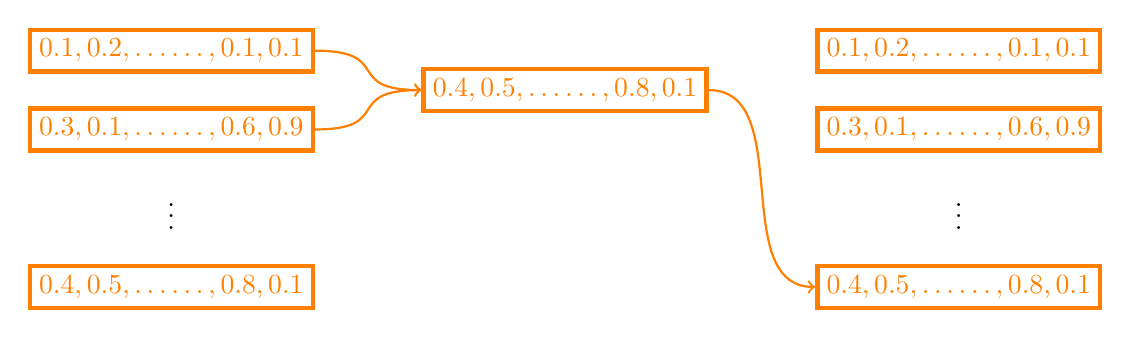
\begin{tikzpicture}
        \node[orange, draw, ultra thick] (0) at (0, 0) {$0.1, 0.2, \dots \dots, 0.1, 0.1$};
        \node[orange, draw, ultra thick] (1) at (0, -1) {$0.3, 0.1, \dots \dots, 0.6, 0.9$};
        \node (2) at (0, -2) {$\vdots$};
        \node[orange, draw, ultra thick] (3) at (0, -3) {$0.4, 0.5, \dots \dots, 0.8, 0.1$};
        \pause
        \node[orange, draw, ultra thick] (4) at (5, -.5) {$0.4, 0.5, \dots \dots, 0.8, 0.1$};
        \draw[orange, looseness=1.8, thick] (0) edge[out=0, in=180, ->, thick] (4);
        \draw[orange, looseness=1.8, thick] (1) edge[out=0, in=180, ->, thick] (4);
        \pause
        \node[orange, draw, ultra thick] (5) at (10, 0) {$0.1, 0.2, \dots \dots, 0.1, 0.1$};
        \node[orange, draw, ultra thick] (6) at (10, -1) {$0.3, 0.1, \dots \dots, 0.6, 0.9$};
        \node (7) at (10, -2) {$\vdots$};
        \node[orange, draw, ultra thick] (8) at (10, -3) {$0.4, 0.5, \dots \dots, 0.8, 0.1$};
        \draw[orange, thick] (4) edge[out=0, in=180, ->, thick] (8);
    \end{tikzpicture}
\end{document}